%%
%% Class homework & solution template for latex
%% Alex Ihler
%%
\documentclass[twoside,11pt]{article}
\usepackage{amsmath,amsfonts,amssymb,amsthm}
\usepackage{graphicx,color}
\usepackage{verbatim,url}
\usepackage{listings}
\usepackage{upquote}
\usepackage[T1]{fontenc}
%\usepackage{lmodern}
\usepackage[scaled]{beramono}
%\usepackage{textcomp}

% Directories for other source files and images
\newcommand{\bibtexdir}{../bib}
\newcommand{\figdir}{figs}

\newcommand{\E}{\mathrm{E}}
\newcommand{\Var}{\mathrm{Var}}
\newcommand{\N}{\mathcal{N}}
\newcommand{\matlab}{{\sc Matlab}\ }

\setlength{\textheight}{9in} \setlength{\textwidth}{6.5in}
\setlength{\oddsidemargin}{-.25in}  % Centers text.
\setlength{\evensidemargin}{-.25in} %
\setlength{\topmargin}{0in} %
\setlength{\headheight}{0in} %
\setlength{\headsep}{0in} %

\renewcommand{\labelenumi}{(\alph{enumi})}
\renewcommand{\labelenumii}{(\arabic{enumii})}

\theoremstyle{definition}
\newtheorem{MatEx}{M{\scriptsize{ATLAB}} Usage Example}

\definecolor{comments}{rgb}{0,.5,0}
\definecolor{backgnd}{rgb}{.95,.95,.95}
\definecolor{string}{rgb}{.2,.2,.2}
\lstset{language=Matlab}
\lstset{basicstyle=\small\ttfamily,
        mathescape=true,
        emptylines=1, showlines=true,
        backgroundcolor=\color{backgnd},
        commentstyle=\color{comments}\ttfamily, %\rmfamily,
        stringstyle=\color{string}\ttfamily,
        keywordstyle=\ttfamily, %\normalfont,
        showstringspaces=false}
\newcommand{\matp}{\mathbf{\gg}}




\begin{document}

\centerline{\Large Homework 1}
\centerline{CS 273A - Machine Learning: Fall \& 2013}
\centerline{\bf Due: 10/3/13}


\subsection*{Problem 3: }
Here is some example matlab code in a listings format:
\begin{lstlisting}
 iris=load('data/iris.txt');     % load the text file
 y = iris(:,end);           % target value is last column
 X = iris(:,1:end-1);       % features are other columns
 whos                       % show current variables in memory and sizes 
\end{lstlisting}

I often need figure formatting and printing functions, which I leave commented out
so they do not appear in the final PDF file, for example (see source latex):
\begin{lstlisting}
 % Some problem solution...
 figure(1);
 plot(X(:,1),X(:,2),'r.', 'markersize',20);   %#
 fname = sprintf('hw_%03d_data.eps', size(X,1));
 set(gca,'fontsize',20);
 print(fname,'-depsc2');  system(['epstopdf ' fname]); system(['rm ' fname]); 
 close all; %#
\end{lstlisting}
The hidden commands create a formatted filename for the output plot, increase the
axes text size, and print the plot.  I personally prefer to output to EPS format,
which has a tight bounding box, and then convert to PDF using a linux command,
but you can also just use the EPS file, or output directly to PDF or another image format.

You can then place figures in the latex file.  In homework and solutions, I prefer to try
to place the figure in-line (``here'') as much as possible, so as to preserve the flow of
code and results.  I also typically lay out figures explicitly with ``tabular'', although
many people prefer to use the subfigure package to do it automatically.
\begin{figure}[h!] \centering
\begin{tabular}{cccc}
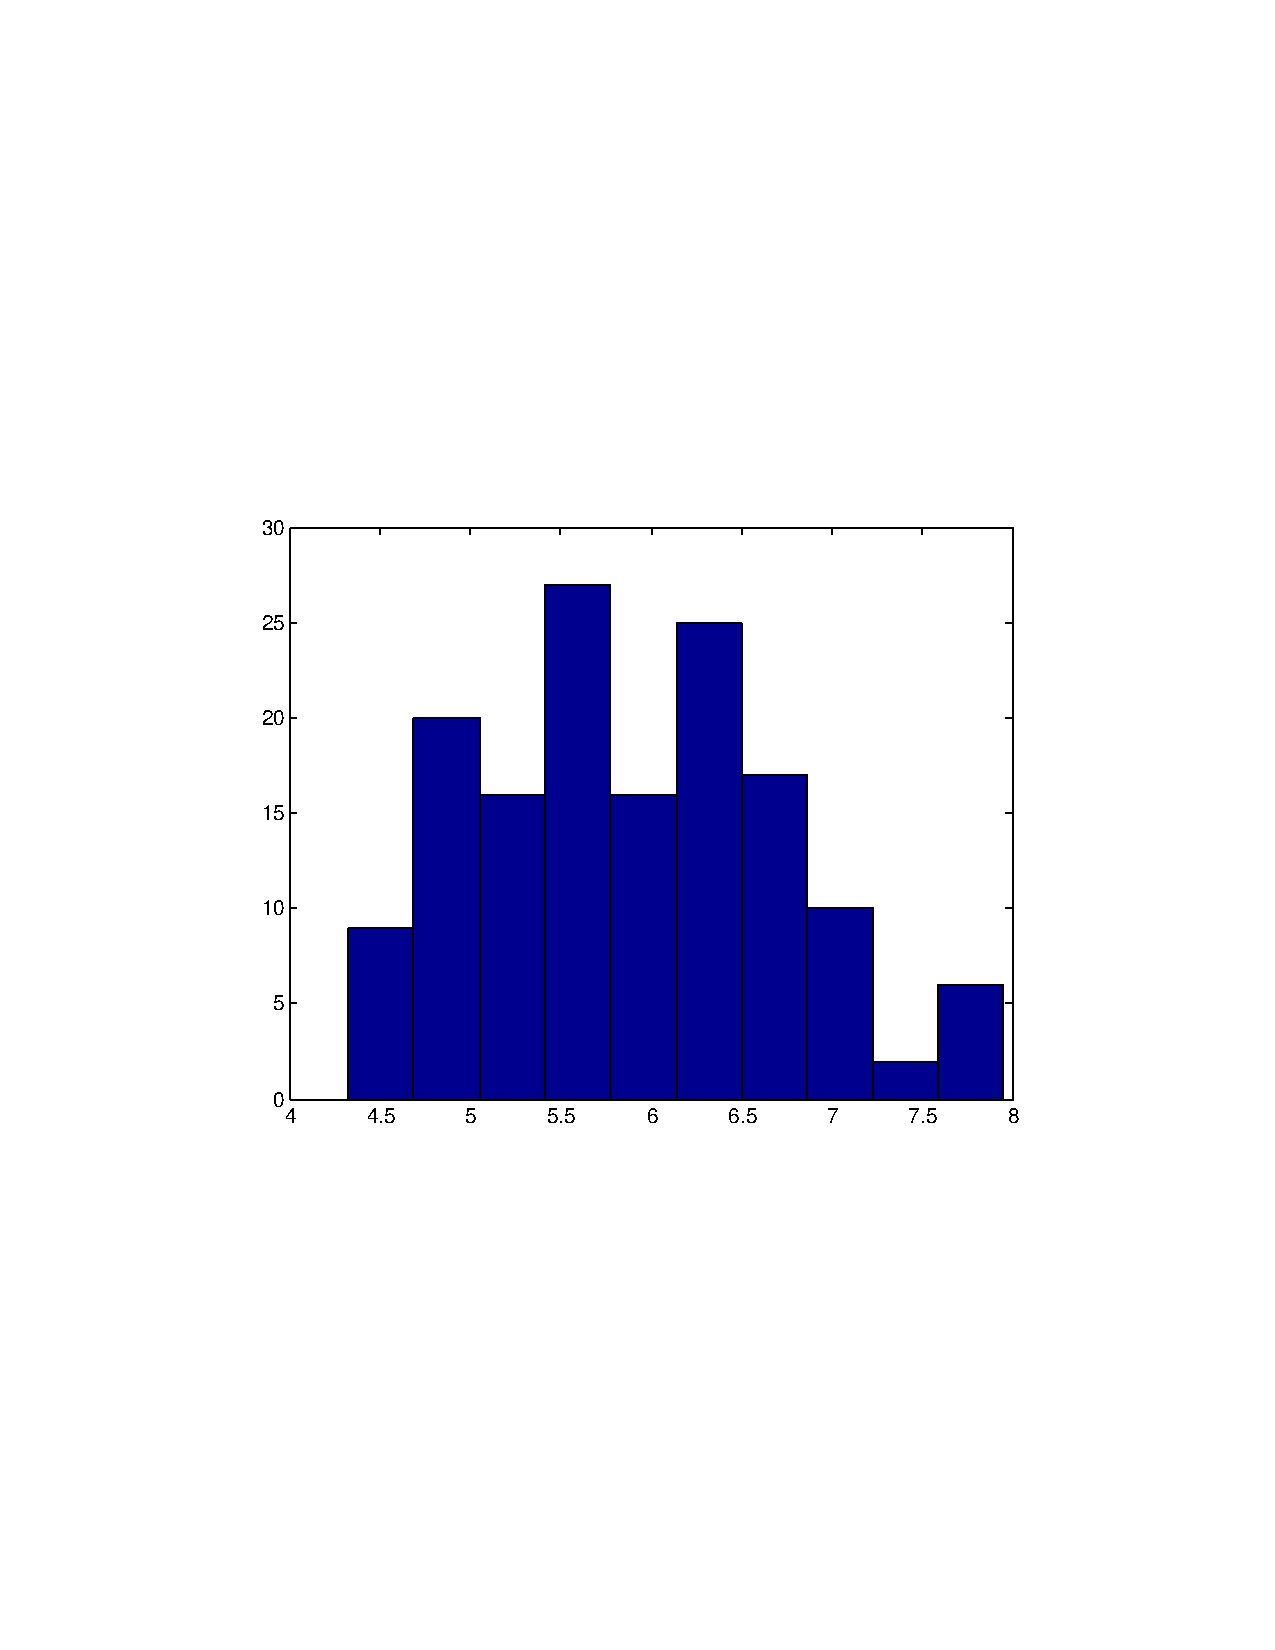
\includegraphics[width=.22\textwidth]{\figdir/iris-feature1} &
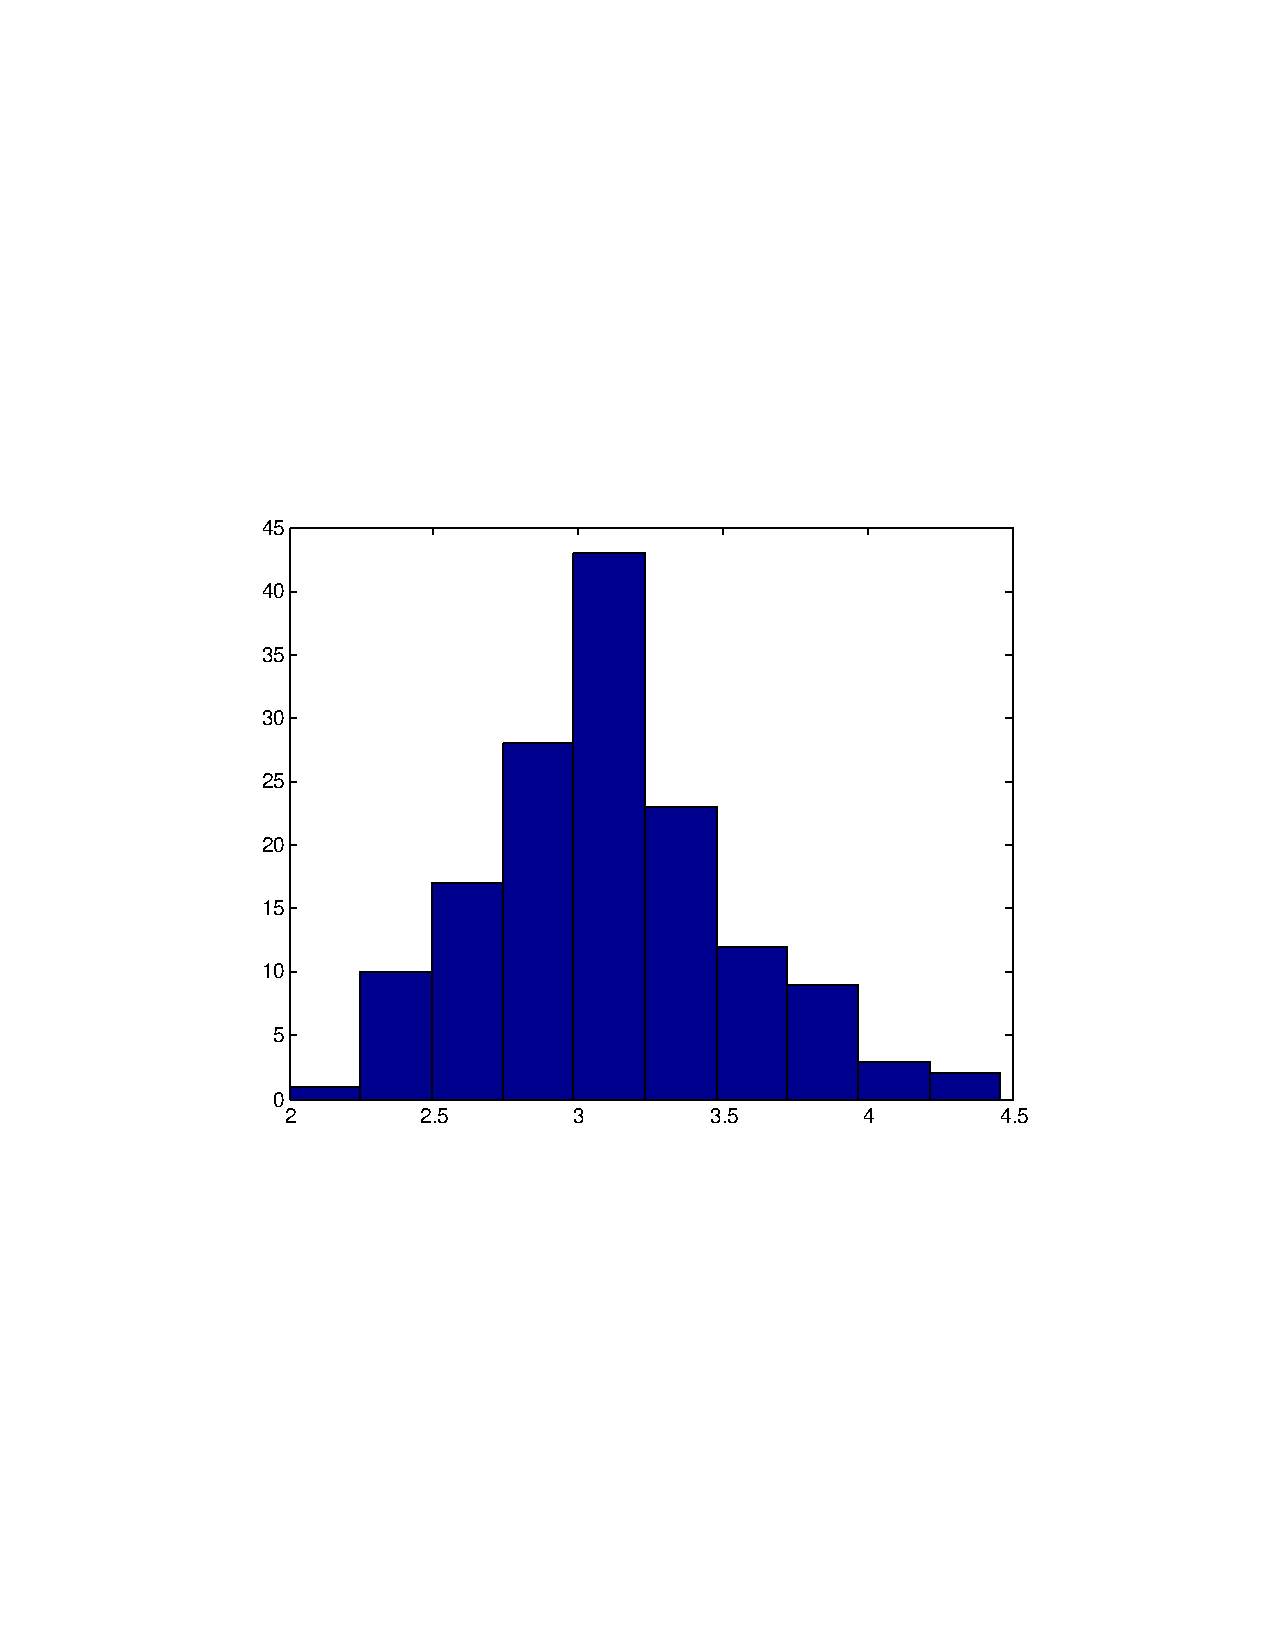
\includegraphics[width=.22\textwidth]{\figdir/iris-feature2} &
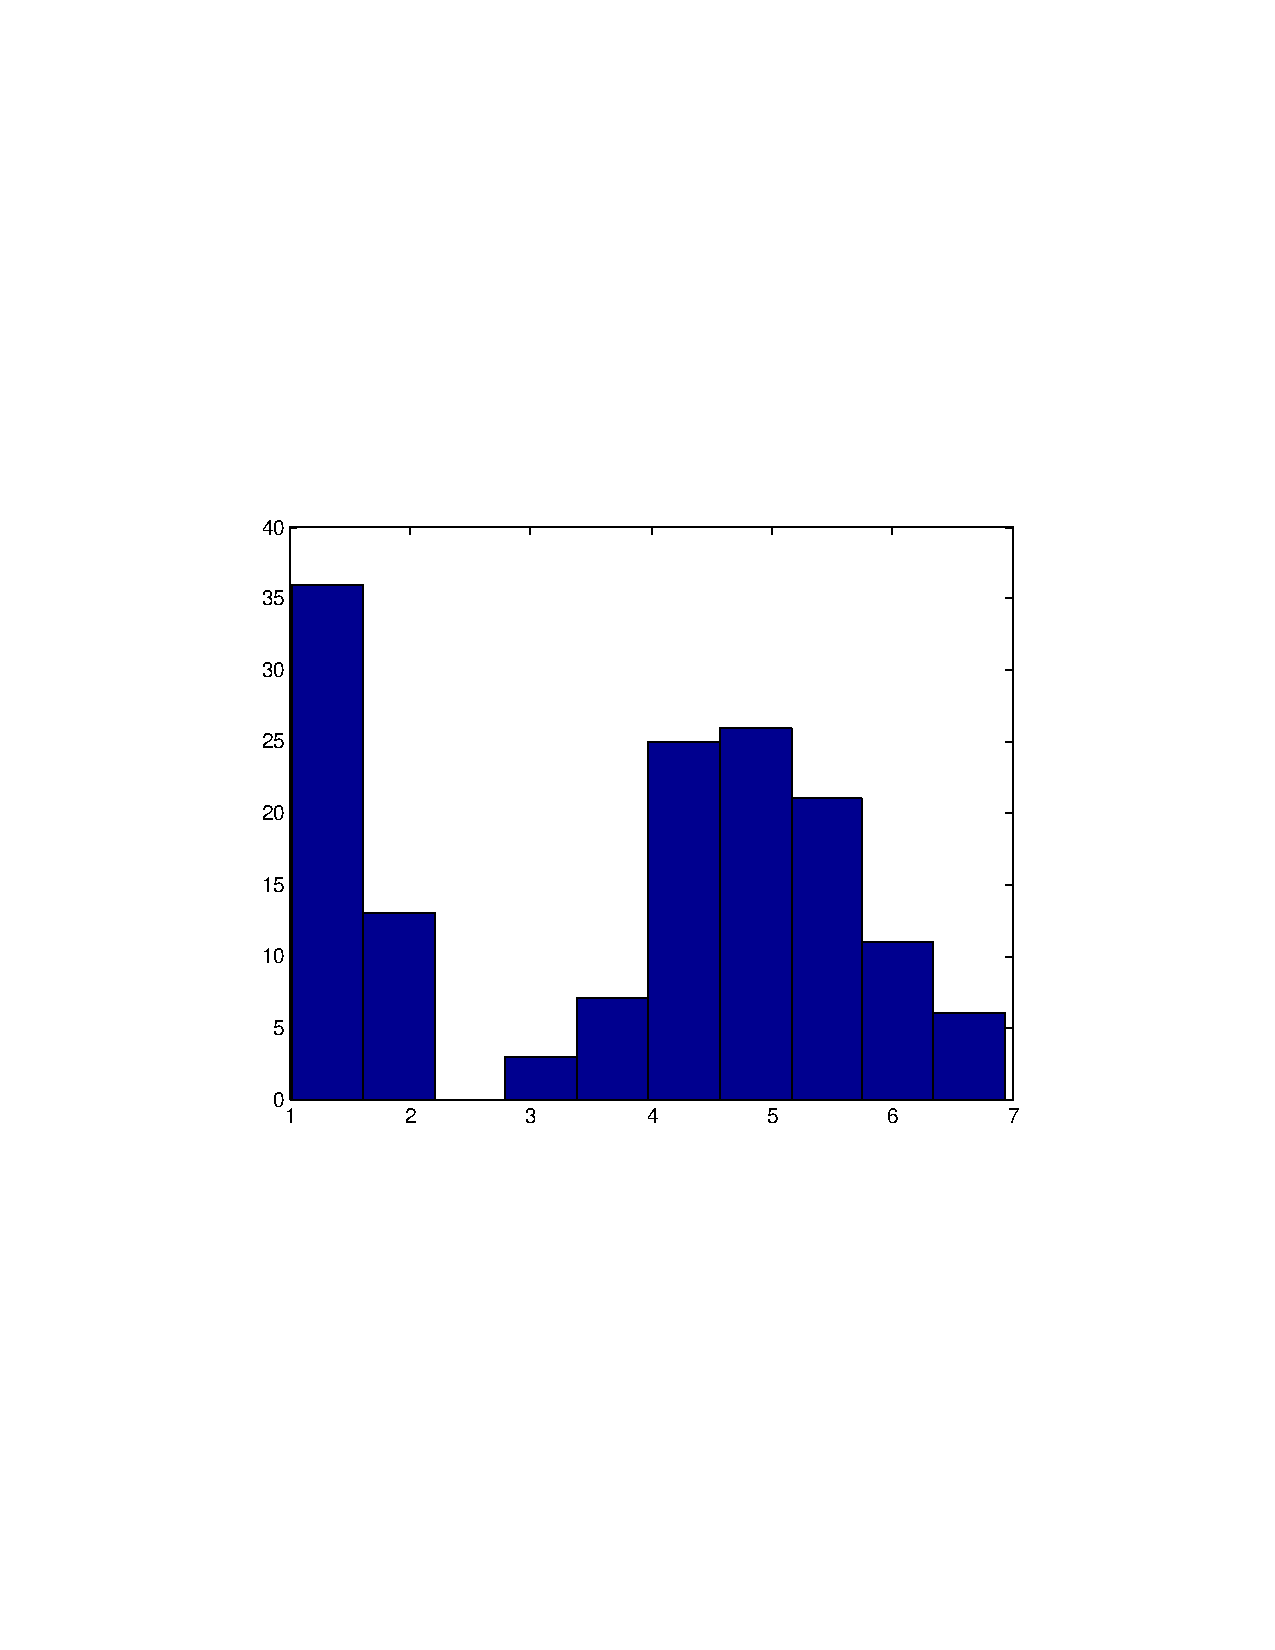
\includegraphics[width=.22\textwidth]{\figdir/iris-feature3} &
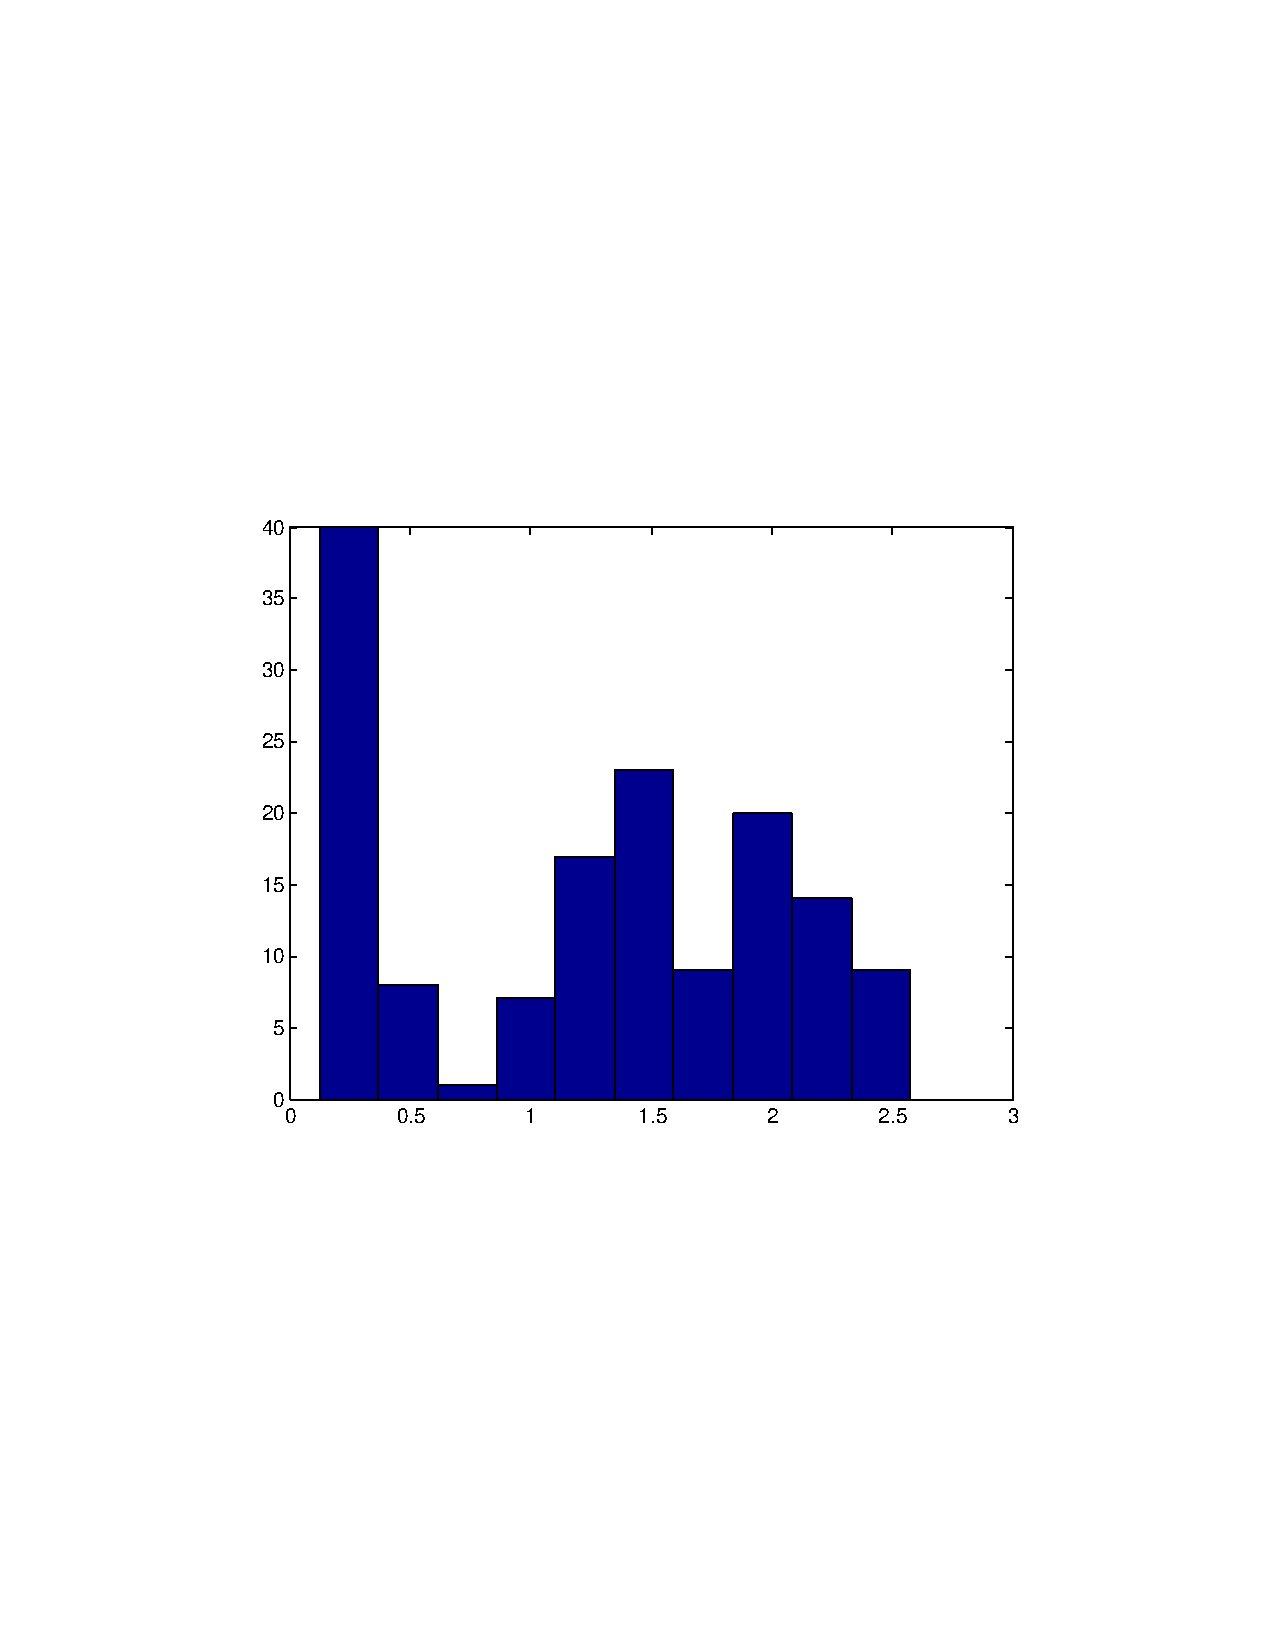
\includegraphics[width=.22\textwidth]{\figdir/iris-feature4} \\
First & Second & Third & Fourth
\end{tabular}
\end{figure}


\end{document}
